%! TEX root = ../main.tex
\documentclass[main]{subfiles}

\begin{document}
\chapter{実験1:MNK問題におけるWalsh関数の予測}
    Walsh関数の代理モデルとしての予測能力を測るために,最適化問題として有名なMNK問題について,Walsh関数を用いて予測する.
    \section{MNK問題}
        \subsection{概要}
        MNK問題\cite{mnk}は各目的の評価関数を最大化する問題である.
        変数間には相関があり,相関のある変数の数を増やすことにより,問題を複雑化することができる.
        MNK問題は,目的数M,設計変数数N,相関のある変数数Kの3つの要素で構成される.
        それぞれの値を変えることによって,問題の複雑度を設定することが出来る.

        \subsection{評価関数}
        \begin{table}[h]
            \centering
            \caption{評価値の例(M=2, N=6, K=1)}
            \begin{tabular}{cc|cc}
              $x_1$ & $x_2$ & $f_1(x_1, x_2)$ & $f_2(x_1, x_2)$\\ \hline
              0 & 0 & 1 & 5 \\
              0 & 1 & 3 & 2 \\
              1 & 0 & 6 & 2 \\
              1 & 1 & 3 & 4 \\
            \end{tabular}
            \label{mnk_table}
        \end{table}
        表\ref{mnk_table}に,M=2,N=2,K=1の時の設計変数と評価値の例を示す.
        $x_1$,$x_2$は変数であり,$f_1(x_1, x_2)$,$f_2(x_2, x_1)$は評価関数である.
        K=1,つまり相関のある変数数が1つなので,自身と相関のある変数が1つある.
        そして,その2つの変数に対して評価値が定義されている.
        M=2であるため,評価関数が2つ設定されている.
        N=6であるため,設計変数は6つ,例えば0,1,0,1,0,1などになる.
        設計変数の1番目と2番目の値を評価関数に入れ評価値を取得する.
        さらに,設計変数の2番目と3番目の値を評価関数に入れ評価値を取得する.
        これを設計変数の5番目と6番目まで繰り返し,評価値の総和を最終的な評価値とする.
    
        \section{実験方法}
        M=2,N=20,K=2の時のMNK問題に対して,まずランダムに生成した入力を20000件用意し,その評価値を求める.
        この20000件のデータの中,ランダムに18000件を選び学習データに,残りの2000件をテストデータにする.
        学習データを用いてWalsh関数を学習させ,パラメータ$w$を決定する.
        学習済みのWalsh関数を用いてテストデータの評価値を予測する.
        実際の正しいテストデータの評価値と比べ,Walsh関数の予測精度を見る.
        予測精度を測る評価指標には決定係数とMAEを用いる.
        また,Walsh関数にはOrder2のものとOrder3のものを使い,Orderの違いによる予測精度の差を確認する.

        \section{結果}
        結果を表\ref{mnk_result}に示す.
        また,正解データと予測データをプロットしたグラフを図\ref{o2},図\ref{o3}に示す.
        \begin{table}[h]
            \centering
            \caption{MNK問題におけるWalsh関数の予測精度}
            \begin{tabular}{c|ccc}
              Order & 計算時間(秒) & 決定係数 & MAE\\ \hline
              2 & $10$ & $0.865$ & $0.0155$ \\
              3 & $51$ & $0.999$ & $5.138 \times 10^{-7}$ \\
            \end{tabular}
            \label{mnk_result}
        \end{table}
        \begin{figure}
          \begin{minipage}[b]{0.45\linewidth}
            \centering
            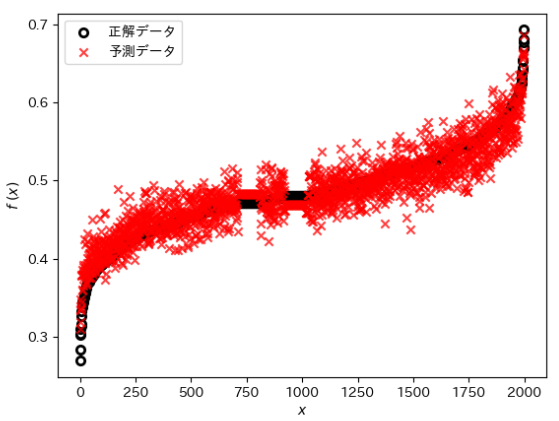
\includegraphics[width=\linewidth]{figures/o2.png}
            \caption{Order2の時の予測データと正解データ}
            \label{o2}  
          \end{minipage}
          \begin{minipage}[b]{0.45\linewidth}
            \centering
            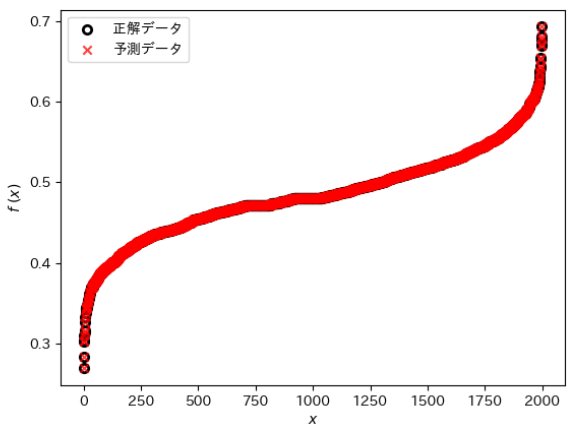
\includegraphics[width=\linewidth]{figures/o3.png}
            \caption{Order3の時の予測データと正解データ}
            \label{o3}
          \end{minipage}
        \end{figure}
        図\ref{o2},図\ref{o3}について,y軸はそれぞれのデータの評価値である.
        このグラフではそれぞれの正解データの評価値を昇順にソートし,小さい方から順に正解データとその予測データの評価値をプロットしている.
        よって,このグラフのx軸はあまり意味を持っていない.
        図\ref{o2},図\ref{o3}を見比べると,Order3の時は全てのデータがほぼ正確に予測できているのに対し,
        Order2では正解データからのばらつきが見られ,Orderの違いによる予測精度の違いが分かる.
        表\ref{mnk_result}を見るとOrder3は決定係数がほぼ1であり,MAEがほぼ0であるため,指標からもほぼ正確に予測できていることが分かる.
        対して,Order2は決定係数が0.865でMAEが0.0155のため,Order3より予測誤差が大きいことが分かる.
        \section{考察}
        結果から,Order3の時,Walsh関数はMNK問題において,ほぼ正確に予測できることが分かった.
        これは,Walsh関数がMNK問題の評価関数をほぼ正確に近似することが出来ている事を表しており,
        Walsh関数が代理モデルとして有用であることを示す1例となったと言える.
        また,Orderが1異なるだけで,予測精度が大きく変わることが分かった.
        よって,精度を高めるにはOrderを増やしていけば良いと言える.
        しかし,表\ref{mnk_result}の計算時間を見ると,Order2とOrder3で5倍ほど計算時間が異なる.
        計算量オーダーは$\mathcal{O}(n!)$であることから,Order4以上では更なる計算時間の増加が考えられる.
        このことから,精度を上げるためにOrderを増やせば良いのではなく,現実的な計算時間で計算が終わるOrderを選択する必要があると言える.
  









\end{document}
